\section{Self-consistent cumulants}

\begin{frame}
    \frametitle{SCCE(GW0) results}
    \begin{figure}
        \centering
        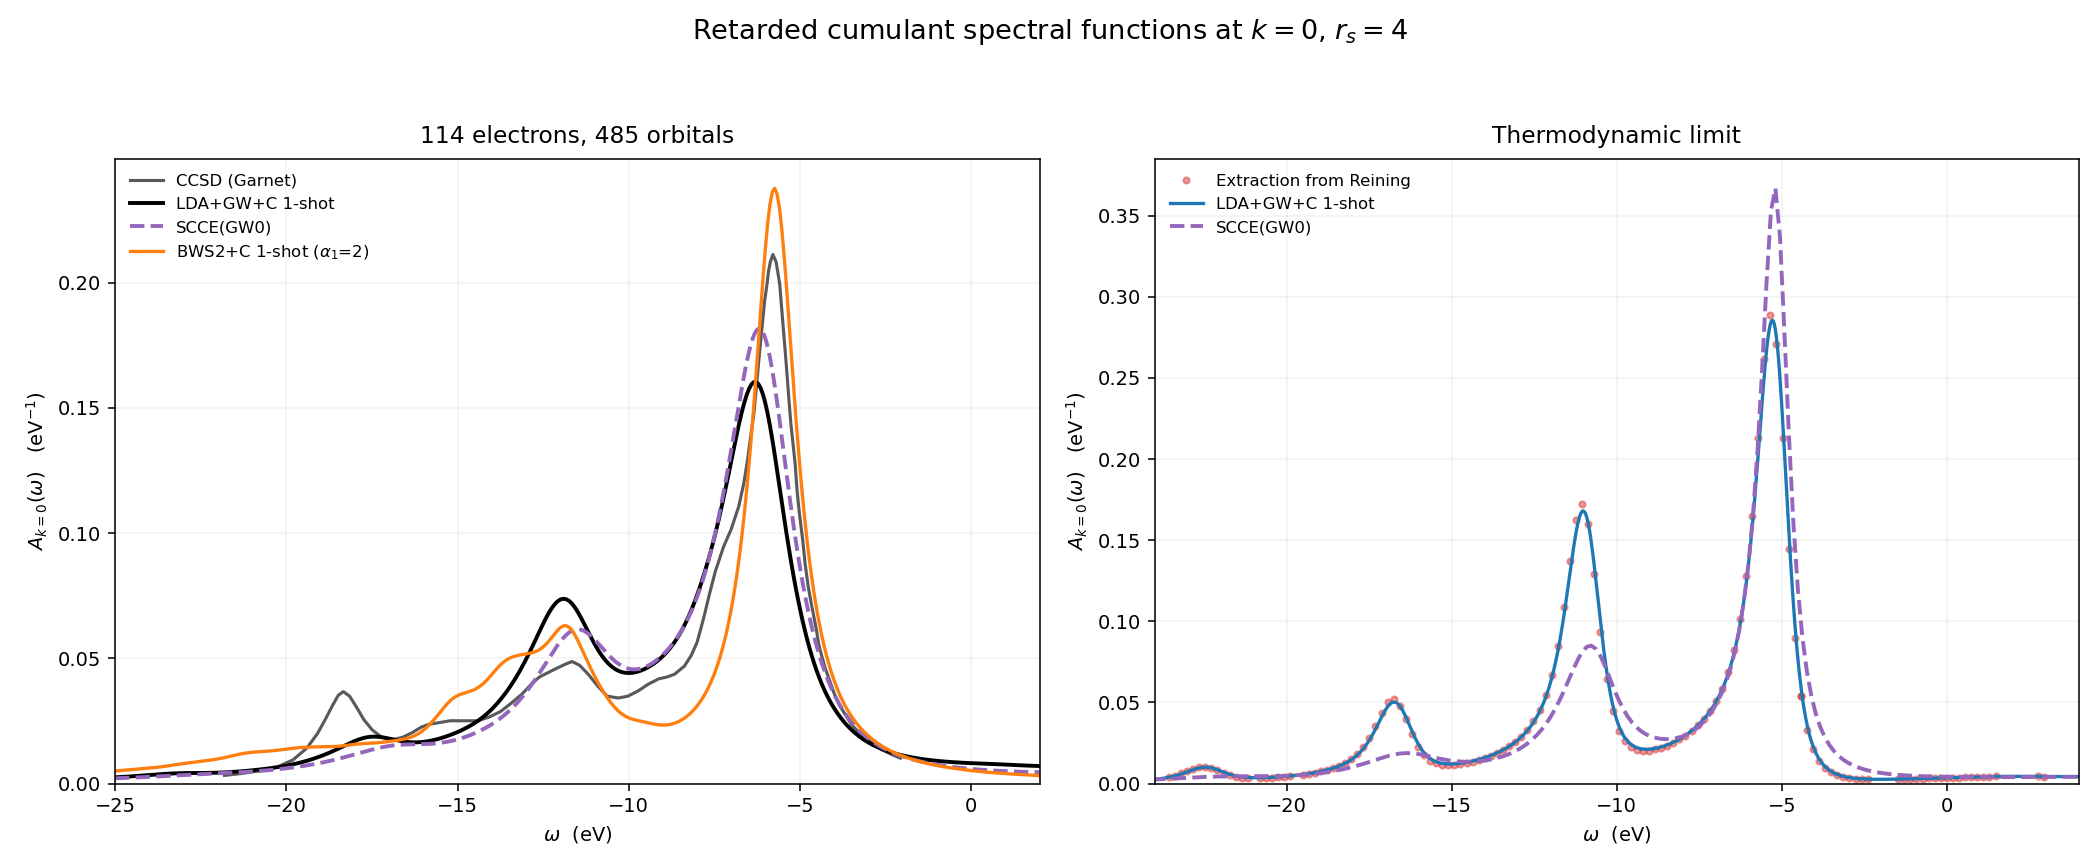
\includegraphics[width=\textwidth]{26/8/8-28/combined_k0_scce.png}
\end{figure}
\end{frame}
\begin{frame}
    \frametitle{SCCE(GW0) theory}
\begin{align} G^{n+1,R}_{k}(t) &= G_{0,k}^{n,R}(t) e^{C_{k}^{n+1,R}(t)}
\label{eq:cumulant_G}\end{align}
where $G_{0,k}^{n,R}(t) = -i \Theta(t) e^{-i \left(k^2/2 + \Gamma_k^{n}\right) t}$ with $\Gamma_k^{0} = V_k^{xc}$. \pause For $n\geq0$,
\begin{equation}
  \Gamma_k^{n+1} = n_{k}^{(n)}v_m+\Sigma_k^{n+1,x(E)}[G^{(n)}]=n_{k}^{(n)}v_m-\sum_{\bm{q}\neq\bm{0}} n_{\bm{k}+\bm{q}}^{(n)}v(\bm{q})  
\end{equation}\pause
After going through the algebra, we arrive at 
\begin{align}
G_k^{n+1,R}(t) &= - i\Theta(t)\, \exp\left[-i \left(k^2/2+\Gamma_k^{n+1}\right) t \right] e^{C_k^{n+1,\text{dyn}}(t)}.
\end{align}\pause
with
 \begin{align}
C_k^{n+1,\text{dyn}}(t) 
% &= \int d\omega\, \beta_{k}^{n+1,R}(\omega)\,\frac{e^{-i\omega t}-1}{\omega^{2}}\\
&= \underbrace{\int\!\dd\omega\,\beta_{k}^{n+1,R}(\omega)
    \frac{e^{-i\omega t}+i\omega t-1}{\omega^2}}_{C^{\rm Landau}_k(t)}
  \;-\; i\,S_1[\beta_k]\,t
\end{align}
where $\beta_{k}^{n+1,R}(\omega)=\frac{1}{\pi}\left|\operatorname{Im}\Sigma_k^{n+1,c}
\!\left(\omega+E_k^{(n)}\right)\right|$ \& $S_1[\beta_k]=\mathcal{P} \int\!\dd\omega\,\frac{\beta_{k}^{n+1,R}(\omega)}{\omega}$.
\end{frame}
\begin{frame}
    \frametitle{Reproduction of PJ's SCCE}
    \begin{figure}
        \centering
        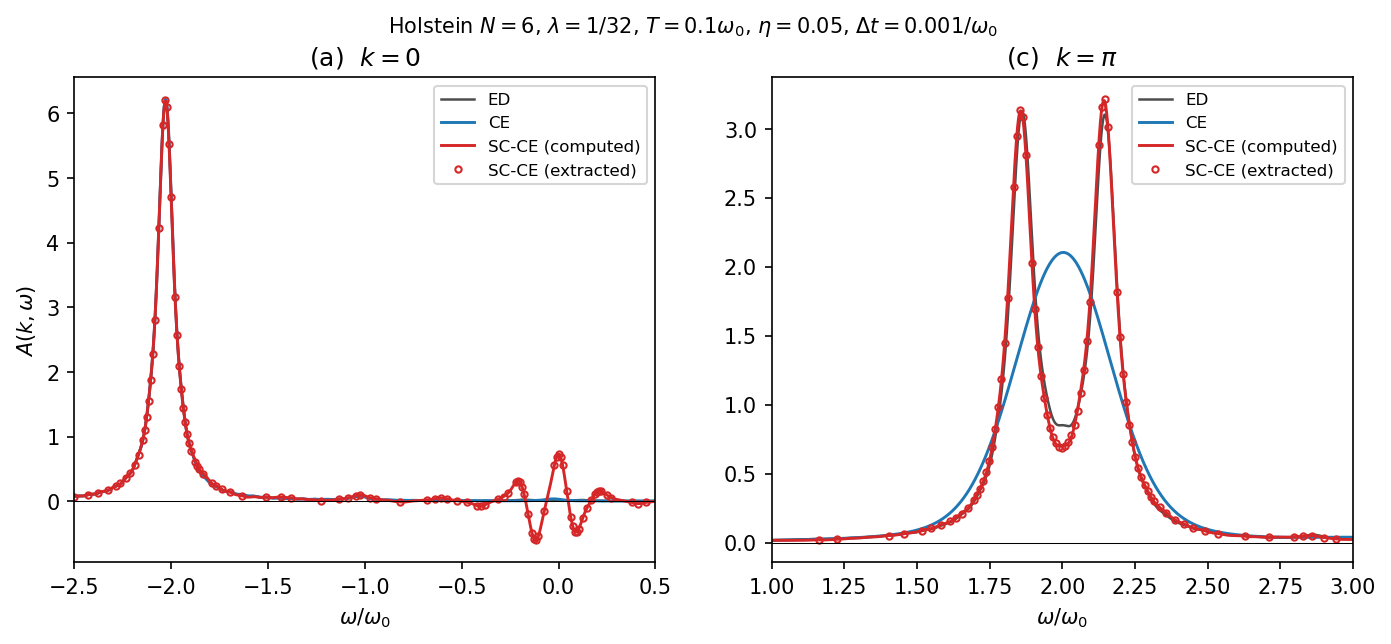
\includegraphics[width=\textwidth]{26/9/9-02/fig1_compare_dt0.001.png}
\end{figure}
\end{frame}
\begin{frame}
    \frametitle{Applying PJ's SCCE to the UEG}
\begin{itemize}
    \item Issue with negative spectral weight \pause
    \item Discuss how to proceed
\end{itemize}
\end{frame}
% \section{Get spectral functions for the UEG via dCC}
\begin{frame}
    \frametitle{Get spectral functions for the UEG via dCC}
\begin{align}
\hat{H}
% &=
% \hat{H}_{\rm el} + \hat{H}_{\rm pl} + \hat{H}_{\rm ep}\\
&= \sum_{{\bm{k}}\in \mathcal{B}} \epsilon_{{\bm{k}}} a_{{\bm{k}}}^{\dagger} a_{{\bm{k}}} + \sum_{\nu_{\bm{q}}\in \mathcal{M}} \omega_{\nu_{\bm{q}}} b_{\nu_{\bm{q}}}^{\dagger} b_{\nu_{\bm{q}}} + \sum_{{\bm{k}}\in \mathcal{B} ; \nu_{\bm{q}}\in \mathcal{M}}g^\nu(\mathbf{k}, \mathbf{q}) a_{{\mathbf{k}+\mathbf{q}}}^{\dagger} a_{{\mathbf{k}}}\left(b_{\nu_{-\mathbf{q}}}^{\dagger}+b_{\nu_{\mathbf{q}}}\right)
\end{align}\pause
Make our zeroth-order reference take on the form
\begin{equation}
    \left|\Phi_0\right\rangle=h_{0}^{\dagger}|0\rangle_{F} \otimes|0\rangle_{B},
\end{equation}
We can define 
\begin{equation}
    \left|\Psi_{\mathrm{CC}}\right\rangle = e^{\hat{T}} \left|\Phi_0\right\rangle,
\end{equation}
% where $\hat{T}^{(1)} = \hat{T}_{\mathrm{el}}^{(1)} + \hat{T}_{\mathrm{pl}}^{(1)} + \hat{T}_{\mathrm{ep}}^{(1)}=0+0+\hat{T}_{\mathrm{ep}}^{(1)}$, \pause
% with
% \begin{align}
% % \hat{T}_{\mathrm{el}}^{(1)}&=\sum^{|\mathrm{k}_i|\neq0}_{|\mathrm{k}_i|<k_F} t_{0}^{\mathrm{k}_i} h_{\mathrm{k}_i}^{\dagger} h_{0}=0 \\
% % \hat{T}_{\mathrm{pl}}^{(1)}&=\sum_{\nu_{\mathrm{q}}} t_{\nu_{\mathrm{q}}} b_{\nu_{\mathrm{q}}}^{\dagger}=0,  \\
% \hat{T}_{\mathrm{ep}}^{(1)}&=\sum_{|\mathrm{k}|<k_F; \nu_{\mathrm{k}}}^{|\mathrm{k}|\neq 0} t_{0, \nu_{\mathrm{k}}}^{\mathrm{k}} h_{\mathrm{k}}^{\dagger} h_{0} b_{\nu_{\mathrm{k}}}^{\dagger}.
% \end{align}
\end{frame}
\begin{frame}
    \frametitle{Cluster operators}
% \begin{align}
% \hat{H}
% % &=
% % \hat{H}_{\rm el} + \hat{H}_{\rm pl} + \hat{H}_{\rm ep}\\
% &= \sum_{{\bm{k}}\in \mathcal{B}} \epsilon_{{\bm{k}}} a_{{\bm{k}}}^{\dagger} a_{{\bm{k}}} + \sum_{\nu_{\bm{q}}\in \mathcal{M}} \omega_{\nu_{\bm{q}}} b_{\nu_{\bm{q}}}^{\dagger} b_{\nu_{\bm{q}}} + \sum_{{\bm{k}}\in \mathcal{B} ; \nu_{\bm{q}}\in \mathcal{M}}g^\nu(\mathbf{k}, \mathbf{q}) a_{{\mathbf{k}+\mathbf{q}}}^{\dagger} a_{{\mathbf{k}}}\left(b_{\nu_{-\mathbf{q}}}^{\dagger}+b_{\nu_{\mathbf{q}}}\right)
% \end{align}\pause
% Make our zeroth-order reference take on the form
% \begin{equation}
%     \left|\Phi_0\right\rangle=h_{0}^{\dagger}|0\rangle_{F} \otimes|0\rangle_{B},
% \end{equation}
% We can define 
% \begin{equation}
%     \left|\Psi_{\mathrm{CC}}\right\rangle = e^{\hat{T}} \left|\Phi_0\right\rangle,
% \end{equation}
$\hat{T}^{(1)} = \hat{T}_{\mathrm{el}}^{(1)} + \hat{T}_{\mathrm{pl}}^{(1)} + \hat{T}_{\mathrm{ep}}^{(1)}=0+0+\hat{T}_{\mathrm{ep}}^{(1)}$
with
\begin{align}
% \hat{T}_{\mathrm{el}}^{(1)}&=\sum^{|\mathrm{k}_i|\neq0}_{|\mathrm{k}_i|<k_F} t_{0}^{\mathrm{k}_i} h_{\mathrm{k}_i}^{\dagger} h_{0}=0 \\
% \hat{T}_{\mathrm{pl}}^{(1)}&=\sum_{\nu_{\mathrm{q}}} t_{\nu_{\mathrm{q}}} b_{\nu_{\mathrm{q}}}^{\dagger}=0,  \\
\hat{T}_{\mathrm{ep}}^{(1)}&=\sum_{\mathrm{k}; \nu_{\mathrm{k}}}^{|\mathrm{k}|\neq 0} t_{0, \nu_{\mathrm{k}}}^{\mathrm{k}} h_{\mathrm{k}}^{\dagger} h_{0} b_{\nu_{\mathrm{k}}}^{\dagger}.
\end{align}\pause
$\hat{T}^{(2)} = \hat{T}_{\mathrm{el}}^{(2)}+\hat{T}_{\mathrm{pl}}^{(2)} + \hat{T}_{\mathrm{ep}}^{(2)}=0+\hat{T}_{\mathrm{pl}}^{(2)} + \hat{T}_{\mathrm{ep}}^{(2)}$ with
% \begin{align}
% \hat{T}_{\mathrm{pl}}^{(2)}&=\frac{1}{2} \sum_{\nu_{\mathrm{q}_1} \nu_{\mathrm{q}_2}} t_{\nu_{\mathrm{q}_1} \nu_{\mathrm{q}_2}} b_{\nu_{\mathrm{q}_1}}^{\dagger} b_{\nu_{\mathrm{q}_2}}^{\dagger}, \\
% \hat{T}_{\mathrm{ep}}^{(2)}&=\sum_{|\mathrm{k}_i|<k_F; \nu_{\mathrm{q}_1} \nu_{\mathrm{q}_2}}^{|\mathrm{k}_i|\neq 0} t_{\nu_{\mathrm{q}_1} \nu_{\mathrm{q}_2}}^{\mathrm{k}_i} h_{\mathrm{k}_i}^{\dagger} h_{0} b_{\nu_{\mathrm{q}_1}}^{\dagger} b_{\nu_{\mathrm{q}_2}}^{\dagger}.
% \end{align}
\end{frame}
